% CHAPTER 1
\chapter{POWER SYSTEM FREQUENCY STABILITY}
\label{chp:2}
The increasing renewable energy penetration deteriorates the power system frequency stability. One of the most severe effect of renewable energy penetration is the reduction in grid inertia. Grid aggregated inertia is important for the frequency stability. As the frequency falls, a part of the kinetic energy is extracted from the grid inertia and released inherently from synchronous generators to grid. Therefore, as the grid aggregated inertia decreases, the control of the frequency becomes difficult resulting in quick changes in the grid frequency.\par
In this chapter, the internal dynamics of the power system will be presented in terms of frequency stability. The frequency regulation mechanisms in the grid are also given. Furthermore, the energy market is briefly explained in order to understand the role of renewable energy providers in the market.
\section{Synchronous Generator and Synchronous Speed}
Synchronous machines produce torque only in synchronous speed. If a transient over-speeding occurs in the rotor, the torque cannot be produced that results in a deceleration. This makes the rotor angular velocity to strictly coupled to the electrical frequency  of the stator rotating MMF. Moreover, these machines are equipped with damper windings which are basically induction machine windings. If the frequency of  grid changes, damper windings create a torque which creates a force to synchronize the speed to the grid frequency. \par
\begin{equation}
n_{s}=\frac{120f}{p}
\label{syncspeed}
\end{equation}
Relation between grid frequency and the synchronous speed is given in Eq. (\ref{syncspeed}) in terms of rpm where $n_{s}$ is the synchronous speed in rpm, $f$ is the grid frequency in Hz, $p$ is the number of poles of the generator \cite{Kundur}.

\section{Swing Equation}
\label{swing}
Rotational speed of synchronous machines changes according to the net torque acting on the rotor. Therefore, the speed is maintained constant unless there is a difference between mechanical and electromechanical torque. The equation of motion is given in Eq. (\ref{eqmotion}) where $J$ is aggravated moment of inertia of the generator and the turbine in $kgm^{2}$, $\omega_{m}$ is the rotor angular velocity in $rad/s$, $T_{m}$ and $T_{e}$ are mechanical and electromechanical torques in $Nm$. $T_{a}$ is the accelerating torque in $Nm$ which determines the acceleration or deceleration in the rotor according to its sign.
\begin{equation}
J\frac{d\omega_{m}}{dt}=T_{m}-T_{e}=T_{a}
\label{eqmotion}
\end{equation}
In power system network, the power ratings of the generators in operation and corresponding moment of inertia values vary. Inertia constant is defined as the ratio of kinetic energy stored in the inertia to the power rating of the generator as in Eq. (\ref{inertiaconstant}) where $\omega_{0m}$ denotes the rated angular velocity of generator in $rad/s$ and $S_{base}$ is the rated apparent power in VA. $H$ indicates the time duration in which generator produces its rated apparent power by only using its kinetic energy in the inertia. Thus, $H$ is a better indication of factor for power system frequency stability analysis compared to $J$. Hence, it is more convenient to use inertia constant, $H$ which varies between 2 and 9 seconds \cite{Kundur}.
\begin{equation}
H=\frac{{\frac{1}{2}}J\omega_{0m}^{2}}{S_{base}}
\label{inertiaconstant}
\end{equation}
Substituting Eq. (\ref{inertiaconstant}) into Eq. (\ref{eqmotion}) and replacing units to per-unit quantities yield the swing equation given in Eq. (\ref{eqmotion5}) where $\overline{P_{m}}$ is the input mechanical power in pu and $\overline{P_{e}}$ is the electromechanical output power in pu. It defines the inherent behaviour of a synchronous generator against the frequency deviations in the grid. When the grid frequency falls, a subsequent decrease in the rotor speed is observed. According to Eq. (\ref{eqmotion5}), a negative term is found in the left-hand side. This means that rotor electromechanical output power, $\overline{P_{e}}$ is increased inherently. It should be noted that the additional energy is not taken from the input mechanical power but it is extracted from the kinetic energy. Moreover, the decreased energy is injected to grid whenever the frequency increases due to the acceleration in the rotor.
%\begin{equation}
%J=\frac{2H}{\omega_{0m}^{2}}{S_{base}}
%\label{inertiaconstant2}
%\end{equation}
%\begin{equation}
%\frac{2H}{\omega_{0m}^{2}}{S_{base}}\frac{d\omega_{m}}{dt}=T_{m}-T_{e}
%\label{eqmotion2}
%\end{equation}
%\begin{equation}
%\frac{2H}{\omega_{0m}^{2}}{S_{base}\omega_{m}}\frac{d\omega_{m}}{dt}=P_{m}-P_{e}
%\label{eqmotion3}
%\end{equation}
%\begin{equation}
%2H\frac{\omega_{m}}{\omega_{0m}}\frac{d(\omega_{m}/\omega_{0m})}{dt}=\frac{P_{m}-P_{e}}{S_{base}}
%\label{eqmotion4}
%\end{equation}
\begin{equation}
2H\overline{\omega_{m}}\frac{d\overline{\omega_{m}}}{dt}=\overline{P_{m}}-\overline{P_{e}}
\label{eqmotion5}
\end{equation}
\section{Frequency in Power Systems}
The frequency in a power system is related to the speed of the synchronous generators and changes according to the swing equation. The frequency of the each generator is not the same in the network since each generator does not have the same speed. Nonetheless, the fluctuations in the generator speeds are called rotor swings and can be negligible in the steady state. Hence, the network can be assumed as a single generating unit by neglecting small differences between the generator speeds. The swing equation basically investigates the relation between mechanical and electromechanical powers and the rate of change of angular speed of a generator. However, it is also applicable to grid in order to estimate the grid frequency.\par
\begin{equation}
\label{systemswing}
2H_{sys}\overline{f}_{sys}\frac{d\overline{f}_{sys}}{dt}=\overline{P}_{tm}-\overline{P}_{te}
\end{equation}
If the generators of the grid are considered as a single generator, the inertia of the equivalent generator is aggregated from each generator in the network. In this case, average frequency in the network can be found as in Eq. (\ref{systemswing}) where $P_{tm}$ is the aggravated mechanical input power of the generators meanwhile $P_{te}$ is the aggravated electromechanical output power. In other words, the system frequency depends on the balance between generation and consumption. It should be noted that generation means the input mechanical power of the generators meanwhile the demand is absorbed from the electromechanical output power of the generators. Hence, the difference between these causes either acceleration or deceleration in the grid frequency. \par
\begin{figure}[h!]
	\centering
	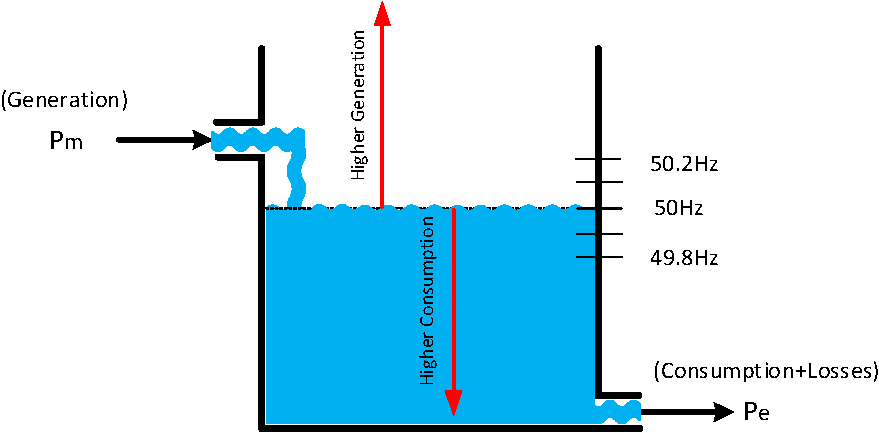
\includegraphics[width=.9\linewidth]{frequencypool.pdf}
	\caption{Frequency Behaviour in Electric Grid with the Water Level in a Container Analogy \cite{Eto2010}}
	\label{frequencyingrid}
\end{figure}
The behaviour of the frequency in electric grid is depicted in Fig. \ref{frequencyingrid}. As it can be seen from the water level in a container analogy, the frequency of the system is dependent on the in-flow and the out-flow. Therefore, in the electricity grid, frequency increases as the aggregated input power is higher than the aggregated output power. Note that, the direction of the frequency is dictated by this balance. Having a constant 49.8Hz frequency does not mean that consumption is higher than generation. If the frequency is constant, then the input mechanical power is equal to output power.\par
The variation of the grid frequency is depicted for a typical day in Fig \ref{06decfreq}. The frequency deviates continuously during the day. It should be noted that there exist hourly peaks in the frequency. The peaks occur due to the change in the hourly generation shift according to the unit commitment. Since the generation level and generating units are changed for the next hour, the frequency deviates hourly in the grid.
\begin{figure}[h!]
	\centering
	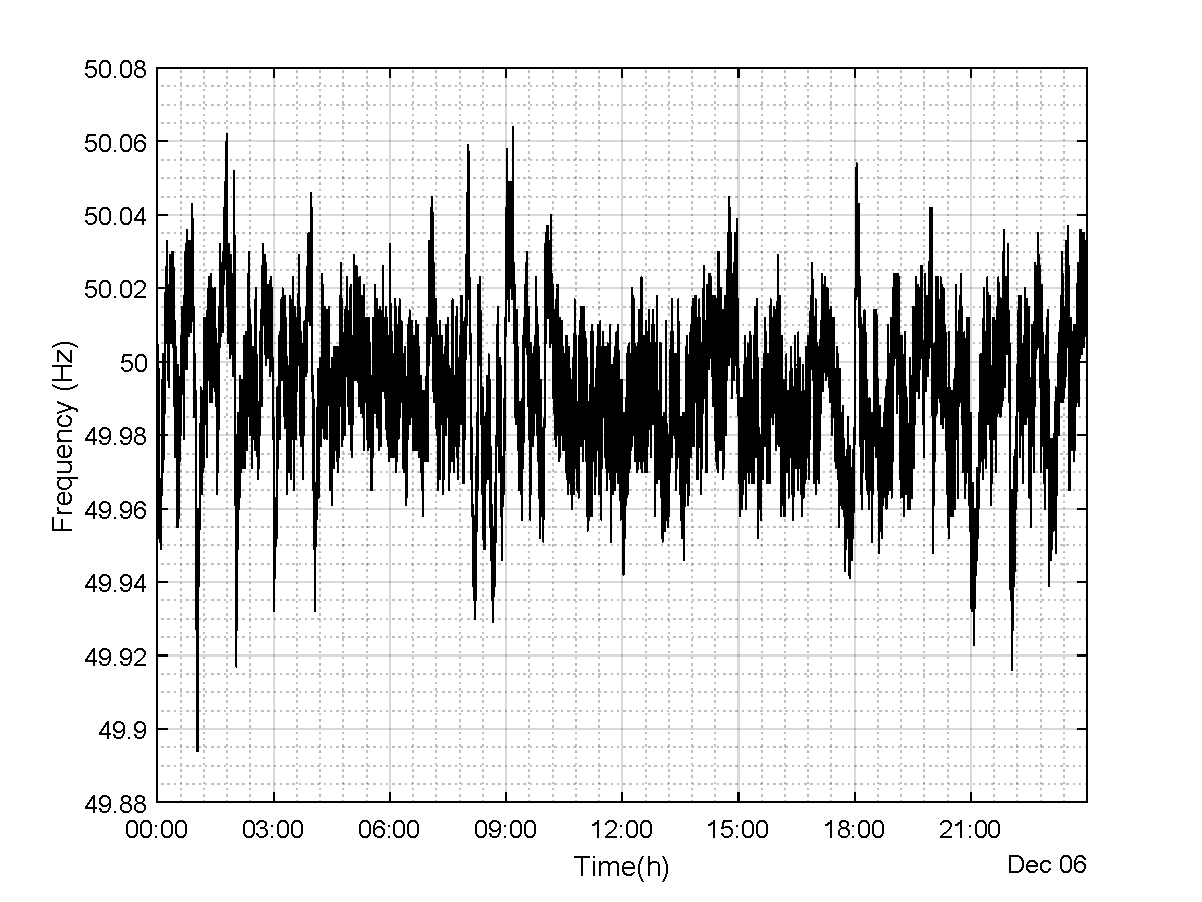
\includegraphics[width=.9\linewidth]{06decfreq.pdf}
	\caption{Variation of the Frequency in a Typical Day (06 Dec 2018) \cite{teiasfreq}}
	\label{06decfreq}
\end{figure}
\section{Frequency Regulating Mechanisms}
Having a constant frequency is one of the most important responsibilities of a system operator. In order to have a constant frequency, supply is being adjusted according to the demand continuously. Consequently, the system frequency varies between a band-gap. The variation in the grid frequency depends on the disturbances which are generally a sudden generation outage or instant load connection. The size of the disturbance determines the severity of the frequency change and there are three main mechanisms to arrest the frequency changes in the system. \par
The frequency control services in England and Wales are depicted in Fig. \ref{freqcontrol} for a frequency disturbance. The frequency is maintained between 49.8Hz and 50.2Hz for continuous service. A frequency disturbance event causes frequency to decline. However, the decline in the frequency is arrested with the help of the inertial support of the conventional generators and the primary frequency controllers. The main responsibility of the primary frequency control is arresting the frequency decline. Restoration of grid frequency to nominal is the responsibility of the secondary and tertiary frequency controls.
\begin{figure}[h!]
	\centering
	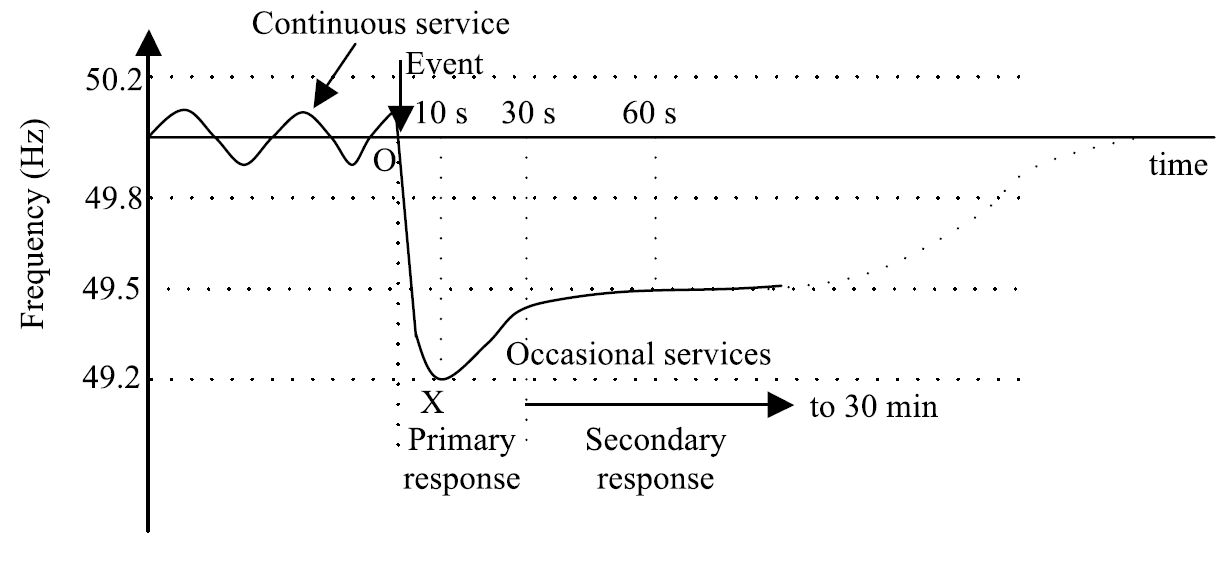
\includegraphics[scale=0.35]{freqq.png}
	\caption{Grid Frequency Control in England and Wales \cite{Ekanayake2008}, \cite{Erinmez1999}}
	\label{freqcontrol}
\end{figure}
\subsection{Primary Frequency Control}
Following a generator outage or a sudden load connection event, frequency starts decreasing. The rate of change of the frequency is dependent on the severity of the event by means of power unbalance and the available inertia of the power system. Such frequency disturbance requires increased input power. However, the increase in the input mechanical power should be activated very fast and should be automated. This responsibility is assigned to generating units with primary frequency control. The active power generation of these units is increased or decreased by the governor depending on the network frequency direction. Notice that each generator in the power system does not necessarily perform primary frequency control function. In this case, their active power generation is independent from the network frequency. The contribution to primary frequency control is a responsibility but also a way to sell higher energy to grid operator.\par
The primary frequency control is automated with droop control defined in the generator speed governors. According to droop control, the generator power should be increased according to the frequency deviation from nominal. Therefore, the generating unit does not utilize its whole capacity but rather keeps a capacity which is called as spinning reserve. According to the droop curve, the generation unit should increase its output power no longer than 15 seconds and keep its operation up to 30 minutes\cite{Machowski2011}.
\subsection{Secondary Frequency Control}
The frequency is recovered back to nominal value with the Secondary Frequency Control action. This controller might be a single or multiple centers that monitor the frequency and adjust the generation accordingly. They are also called as Automatic Generation Control (AGC) systems and their action takes a few minutes. AGC monitors the frequency deviation from the nominal and takes action to recover frequency back to nominal. With the secondary frequency control action, primary controllers decrease their production back to their pre-disturbance value.
\subsection{Tertiary Frequency Control}
The final frequency control mechanism is the Tertiary Frequency Control. If the frequency is not recovered back to nominal value with the secondary controllers, tertiary frequency controllers manually activate the load shedding which is an undesired situation by the network operator. However, it is an emergency case which might result in black-out and requires immediate action.
\section{Energy Market}
Since the energy is generated and distributed by private energy companies, a system operator should be responsible for maintaining a balance in the power network. The frequency is kept inside the operational band in the electricity network by balancing the supply and the demand by intersecting the supply and demand curves inside the different time intervals. In this way, the balance is ensured in the market by day ahead, intra-day and balancing markets. 
\subsection{Day Ahead Market}
The load power in a network has a distinct characteristic depending on the day of the week or the hour of the day. By foreseeing the next day demand power variation, the electricity market collects the bids from the energy suppliers and consumers. According to submitted bids, the next day generation price is determined by intersecting the supply and demand price curves. The price of the energy is called Market Clearing Price (MCP). These bids are submitted for the next day and the prices are determined before the corresponding day.
\subsection{Intra-Day Market}
Even though the estimations for the upcoming day load power has significant accuracy with the advanced estimation methods, networks are subjected to unexpected problems such as generator trips, line outages. Therefore, intra-day market contributes the balance of the market between the day ahead market and balancing market. Moreover, it gives the participants almost real-time trading opportunity meanwhile it increases the sustainability of the market. After day ahead market has closed for the corresponding day, the bids are submitted to system. In other words, MCP is already determined for the corresponding day meanwhile the rest of the day prices are not set. The average of the bids submitted to market is called as Weighted Average Price (WAP).
\subsection{Balancing Market}
Primary and secondary control reserves are maintained in the system in order to improve the balance for the instant deviations in the frequency. The frequency is first arrested by the primary controllers and it is restored by the secondary controllers. The generation units that participate primary and secondary control promise a defined generation capacity to these actions. Balancing market is much more different than day ahead and intra-day market since its main goal is the network security rather than electricity trading. The price of the energy in this market called as System Marginal Price (SMP).\par
The price of the energy changes according to the market type. In Fig. \ref{markets}, three market prices such as Market Clearing Price (MCP), Weighted Average Price (WAP) and System Marginal Price (SMP) are shown for a typical day. MCP and WAP are close to each other since they are scheduled much before operation time. Nevertheless, SMP fluctuates more since it is the resultant price of the balancing market. Notice that balancing market price might be higher than day ahead and intra-day prices. However, balancing market is not appropriate platform for trade purposes due to the fact that main object in this market is the successful operation of the system.
\begin{figure}[h!]
	\centering
	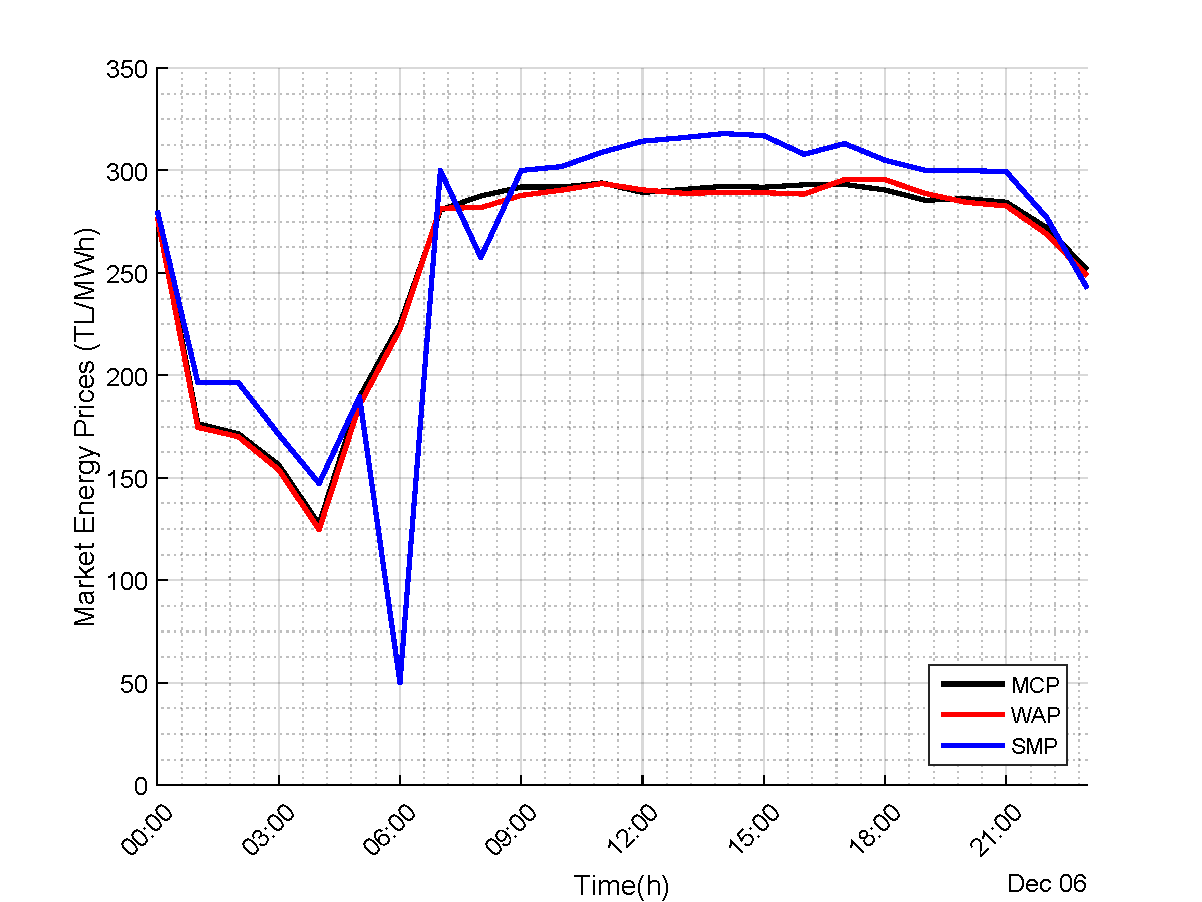
\includegraphics[scale=0.7]{marketprices.pdf}
	\caption{Energy Prices on 06 Dec. 2018 \cite{TEIAS2019}}
	\label{markets}
\end{figure}
\subsection{Feed-In Tariff}
\label{section-price}
Significant amount of energy produced inside the Turkish electricity network is based on exported sources such as coal and gas. As a result of this, the energy sector is highly dependent on foreign countries. In order to decrease the dependency on the external sources, the renewable energy sources are supported by government in Turkey. The energy generated by renewable energy systems are sold with the feed-in tariff (FIT) within the pre-determined time interval according to the purchase agreement. This decreases the return of investment due to the fact that all produced energy will be sold during this period with a remarkable price. The feed-in tariff for different renewable energy systems is listed in Table \ref{price}.\par
\begin{table}[h]
	\centering
	\begin{tabular}{cc}
		\hline
		\textbf{Renewable Energy System} & \textbf{\begin{tabular}[c]{@{}c@{}}Feed-In Tariff\\ (cent/kWh)\end{tabular}} \\ \hline
		Hydro                            & 7.3                                                                          \\
		Wind                             & 7.3                                                                          \\
		Geothermal                       & 10.5                                                                         \\
		Biomass                          & 13.3                                                                         \\
		Solar                            & 13.3                                                                         \\ \hline
	\end{tabular}
\caption{Feed-In Tariff for Renewable Energy Systems in Turkey \cite{yasa}}
\label{price}
\end{table}
In addition to feed-in tariff, energy provider can benefit from additional incentives as long as some parts of the system is produced inside Turkey. For instance, by choosing a tower of a wind turbine which is a domestic production, an additional price is given to energy provider as local-bonus content. The local-bonus contents for wind turbines are listed in Table \ref{price2}.\par
\begin{table}[h!]
	\centering
	\begin{tabular}{cc}
		\hline
		\textbf{\begin{tabular}[c]{@{}c@{}}Local Content\\ for Wind Turbines\end{tabular}}   & \textbf{\begin{tabular}[c]{@{}c@{}}Local Content Incentive\\ (cent/kWh)\end{tabular}} \\ \hline
		Blade                                                                                & 0.8                                                                                   \\
		\begin{tabular}[c]{@{}c@{}}Generator and \\ Power Electronics\end{tabular}           & 1.0                                                                                   \\
		Turbine Tower                                                                        & 0.6                                                                                   \\
		\begin{tabular}[c]{@{}c@{}}All Mechanical Parts in \\ Rotor and Nacelle\end{tabular} & 1.3                                                                                   \\ \hline
	\end{tabular}
	\caption{Local Content Incentives for Wind Turbines\cite{yasa}}
	\label{price2}
\end{table}
With the increasing renewable energy penetration, the power system stability is getting more vulnerable to the disturbances. Since the grid operators are responsible for the successful operation of the grid, they have to work in order to improve the grid stability. Meantime, maintaining power system stability is not a responsibility of the energy providers. However, participation of the renewable energy providers is also a necessity to improve frequency stability of the grid. Hence, the grid operators have to come up with a solution to be implemented by the energy providers. Nonetheless, the solution should also be beneficial for the energy providers which are already satisfied with the existing purchase agreement with additional incentives. As long as the renewable energy providers are convinced to implement the solutions, the grid stability can be maintained against the increasing renewable penetration.
\section{Conclusion}
This chapter focuses on the frequency dynamics inside the power grid. The importance of the synchronous generators on the frequency is investigated by focusing on the inertial support behaviour. The characteristic of the inertial support is explained with the swing equation. The frequency behavior of the electricity grid is explored according to the supply and demand relation. \par
Grid frequency is maintained around the nominal frequency with the help of the frequency regulating mechanisms. Primary, secondary and tertiary frequency control mechanisms are briefly explained. In addition to technical details, the energy market is also summarized to present an economical perspective. Notice that economical aspect is also important for the feasibility of the inertial support that is expected to be implemented by energy providers.